\section{Literature Review}
The advent of "modern" object detection has enabled more sophisticated and automated methods for understanding visitor engagement and flow in cultural institutions. This literature review aims to explore the current state of research on object detection and visitor behaviour analysis in cultural institutions, focusing on privacy-preserving techniques, dataset specialization for enhanced object detection accuracy, and case studies of technology implementation.

\subsection{Analysis of Traditional and Technological Methods for Visitor Behavior Studies}

Studies on traditional methods of analyzing visitor behavior\footnote{Traditional methods include surveys, manual counting, and direct observation} reveal both their use cases and limitations.

\citeauthor{la2017museumbehaviouranalysis} explored alternative technological approaches in their study on museum visitor behavior and its perceived value to museum curators (\citeyear{la2017museumbehaviouranalysis}). Wearable RFID trackers were given to the visitors, and beacons were positioned at positions deemed important by the museum curators. The beacons would then communicate the positions of the visitors to the system. This allowed for the collection of data on key metrics like exhibit popularity, average visit duration, and common visitor paths. They noted that technology-based visitor behavior analysis was generally well-received by museum curators, offering valuable data that could enhance the visitor experience.

However, the requirement for visitors to wear RFID trackers represents a significant drawback, as it may be perceived as intrusive (although completely privacy preservant).

The study of \citeauthor{la2017museumbehaviouranalysis} also highlighted divergent views on the utility of visitor behavior analysis systems (\citeyear{la2017museumbehaviouranalysis}). Administrators and department heads generally viewed these systems favorably, citing the financial justification for expensive exhibitions: "We really need to know if this expenditure was worthwhile" (\cite{la2017museumbehaviouranalysis}). On the contrary, museum curators expressed skepticism. One curator remarked, "A temporary exhibition won’t change after you deploy it, and understanding how it is used by the public would not help me in my next exhibition, since they are each very different. My main reason to analyze behavior would be to satisfy my curiosity." This contrast underscores the varied perspectives within museums regarding the value and implications of behavior analysis technologies.

\subsection{Privacy}
\label{sec:lit-privacy}
Section \ref{sec:lit-privacy}, is a rewritten and improved version of the same section in an unpublished pre-thesis project written by the same candidate as this master thesis.

\subsubsection{The General Data Protection Regulation}
\label{sec:GDPR}
This section serves as a summarization of some aspects of the GDPR relevant to the thesis.

The GDPR entered into applicability in the EU on 25th of May 2018 as a way for people to have more control over their data, and for having a level playing field for all companies. There is now one set of data protection rules for all companies operating in the European Economic Area (EEA). The EEA consists of all EU countries plus Iceland, Liechtenstein and Norway. The most relevant parts of the GDPR are the regulations regarding personal data.

\paragraph{Personal Data}
\label{sec:personal_data}
Personal data is any form of information that can be connected to an identifiable data subject. The following definition was given by the european parliament in 2016:

\begin{myquote}{Definition of personal data, as given by EUs GDPR}
    "The term 'personal data' means any information relating to an identifed or identifable natural person ('data subject'); an identifable natural person is one who can be identifed, directly or indirectly, in particular by reference to an identifer such as a name, an identifcation number, location data, an online identifer or to one or more factors specifc to the physical, physiological, genetic, mental, economic, cultural or social identity of that natural person" (\cite{in2023gdpr_website}).
\end{myquote}

Regulations regarding personal data also applies to the events where pieces of information are aggregated to identify a person. It is possible to store information about individuals without it being personal data. This can be done in several ways, one of them being by the method of differential privacy. Differential privacy is explained in section \ref{sec:differential-privacy}.

Another approach to the personal data is to process it the right way.

\paragraph{Legal Bases for Processing Personal Data}
\label{sec:legal-bases-processing-personal-data}
Processing of personal data is permissible under the GDPR only when it satisfies at least one of the following legal bases:
\begin{enumerate}
    \item The data subject has given explicit consent.
    \item It is necessary for the performance of a contract to which the data subject is a party.
    \item It is necessary for compliance with a legal obligation to which the controller is subject.
    \item It is necessary to protect the vital interests of the data subject or of another natural person.
    \item It is necessary for the performance of a task carried out in the public interest or in the exercise of official authority vested in the controller.
    \item It is necessary for the purposes of the legitimate interests pursued by the controller or by a third party, except where such interests are overridden by the interests or fundamental rights and freedoms of the data subject which require protection of personal data.
\end{enumerate}

Additionally, the controller is 1) responsible for compliance with the 3 requirements summarized below, and 2) should be able to demonstrate this compliance at any given time.

\begin{enumerate}
    \item{Security Documentation}
          In the event of a breach of personal data, the controller must document that proper precautions were made to secure the data. One of these precautions is to deleted data that is no longer needed. This rule to delete no-longer-needed data is often overlooked and violated by companies (\cite{sa2022webinar_gdpr}).
    \item{Data breaches}
          Breaches of personal data must be reported within 72 hours. Companies failing to do so are economically sanctioned, but even worse, it damages the reputation of the company. In such cases it is common to uncover more failures (\cite{sa2022webinar_gdpr}). This is often that the company has failed to make, or failed to document, the efforts they have made to sufficiently protect the data (the first requirement).
    \item{Rights of the data subject}
          The data subject has the right to be informed about how their personal data is handled. This is commonly achieved through the company's privacy declaration, which must be comprehensive and regularly updated. Additionally, companies are encouraged to proactively communicate this information to clients, for instance, via email. According to privacy experts (\cite{sa2022webinar_gdpr}), adopting such practices is an effective way of building and maintaining trust with customers.
\end{enumerate}

\paragraph{The NIS2 Directive}
\label{sec:NIS2_relevance}

The NIS2 Directive (\cite{eu2022nis2}) is a more recent EU regulation that came into force in January 2023. Unlike the GDPR, which broadly addresses the protection of personal data, NIS2 is specifically targeted toward technology. As an update to the EU's cybersecurity framework, NIS2 focuses on strengthening the security of network and information systems throughout the Union. It emphasizes the critical need for robust security measures in systems that process personal data to prevent unauthorized access and data leaks.

Both NIS2 and GDPR highlight the principle of data minimization, which mandates that object detection systems process only the necessary amount of personal data for their intended function. This practice not only bolsters security but also supports privacy by minimizing potential data exposure. Adhering to these principles is vital for maintaining user trust and ensuring compliance with EU regulations, particularly when deploying object detection technologies in environments where data sensitivity is paramount.

\subsubsection{Preservation of Individual Privacy}

Preservation of individual privacy refers to maintaining the personal space and confidentiality of individuals, ensuring that their private lives and personal integrity are not invaded or exposed without consent. This involves considerations beyond just data, including behaviors and surveillance. Protection of personal data specifically deals with the management and security of personal information—data that can identify an individual, such as names, addresses, and biometrics. This protection is primarily about the correct handling, processing, storage, and destruction of personal data to prevent unauthorized access, misuse, or breaches. While protection of personal data is important due to the regulations, preserving the individual privacy is essential in object detection of persons.

There are multiple methods, both pre- and post-processing, for preserving individual privacy. One example of a pre-processing privacy preservation method is to hide the facial regions optically during capture, which was done in a study on fall detection by \citeauthor{wa2020elderly_fall_detection_meta} (\citeauthor{wa2020elderly_fall_detection_meta}).

Post-processing methods include various techniques to obscure identifiable information after the data has been captured. These range from simple blurring and pixelation to more sophisticated approaches such as k-anonymity (\cite{sw2002kAnonymity}) and differential privacy. Six of the simple, easy-to-implement methods are shown in figure \ref{fig:obfuscation_methods}, demonstrating practical implementations.

K-anonymity claimed to be a mathematically proven method for anonymyzation of personal data, but has been critizised by it's successor, the l-diversity criterion, for not being robust in the events where attackers have background data (ma2007l-diversity). Differential privacy is a statistical disclosure control algorithm to process individual data from a group to produce close-to-real outcomes without disclosing the personal data of individuals (\cite{hu2023metaverse-privacy}). Differential privacy is explained and illustrated in \ref{sec:differential-privacy}.

\begin{figure}[H]
    \centering
    \begin{subfigure}{0.46\textwidth}
        \centering
        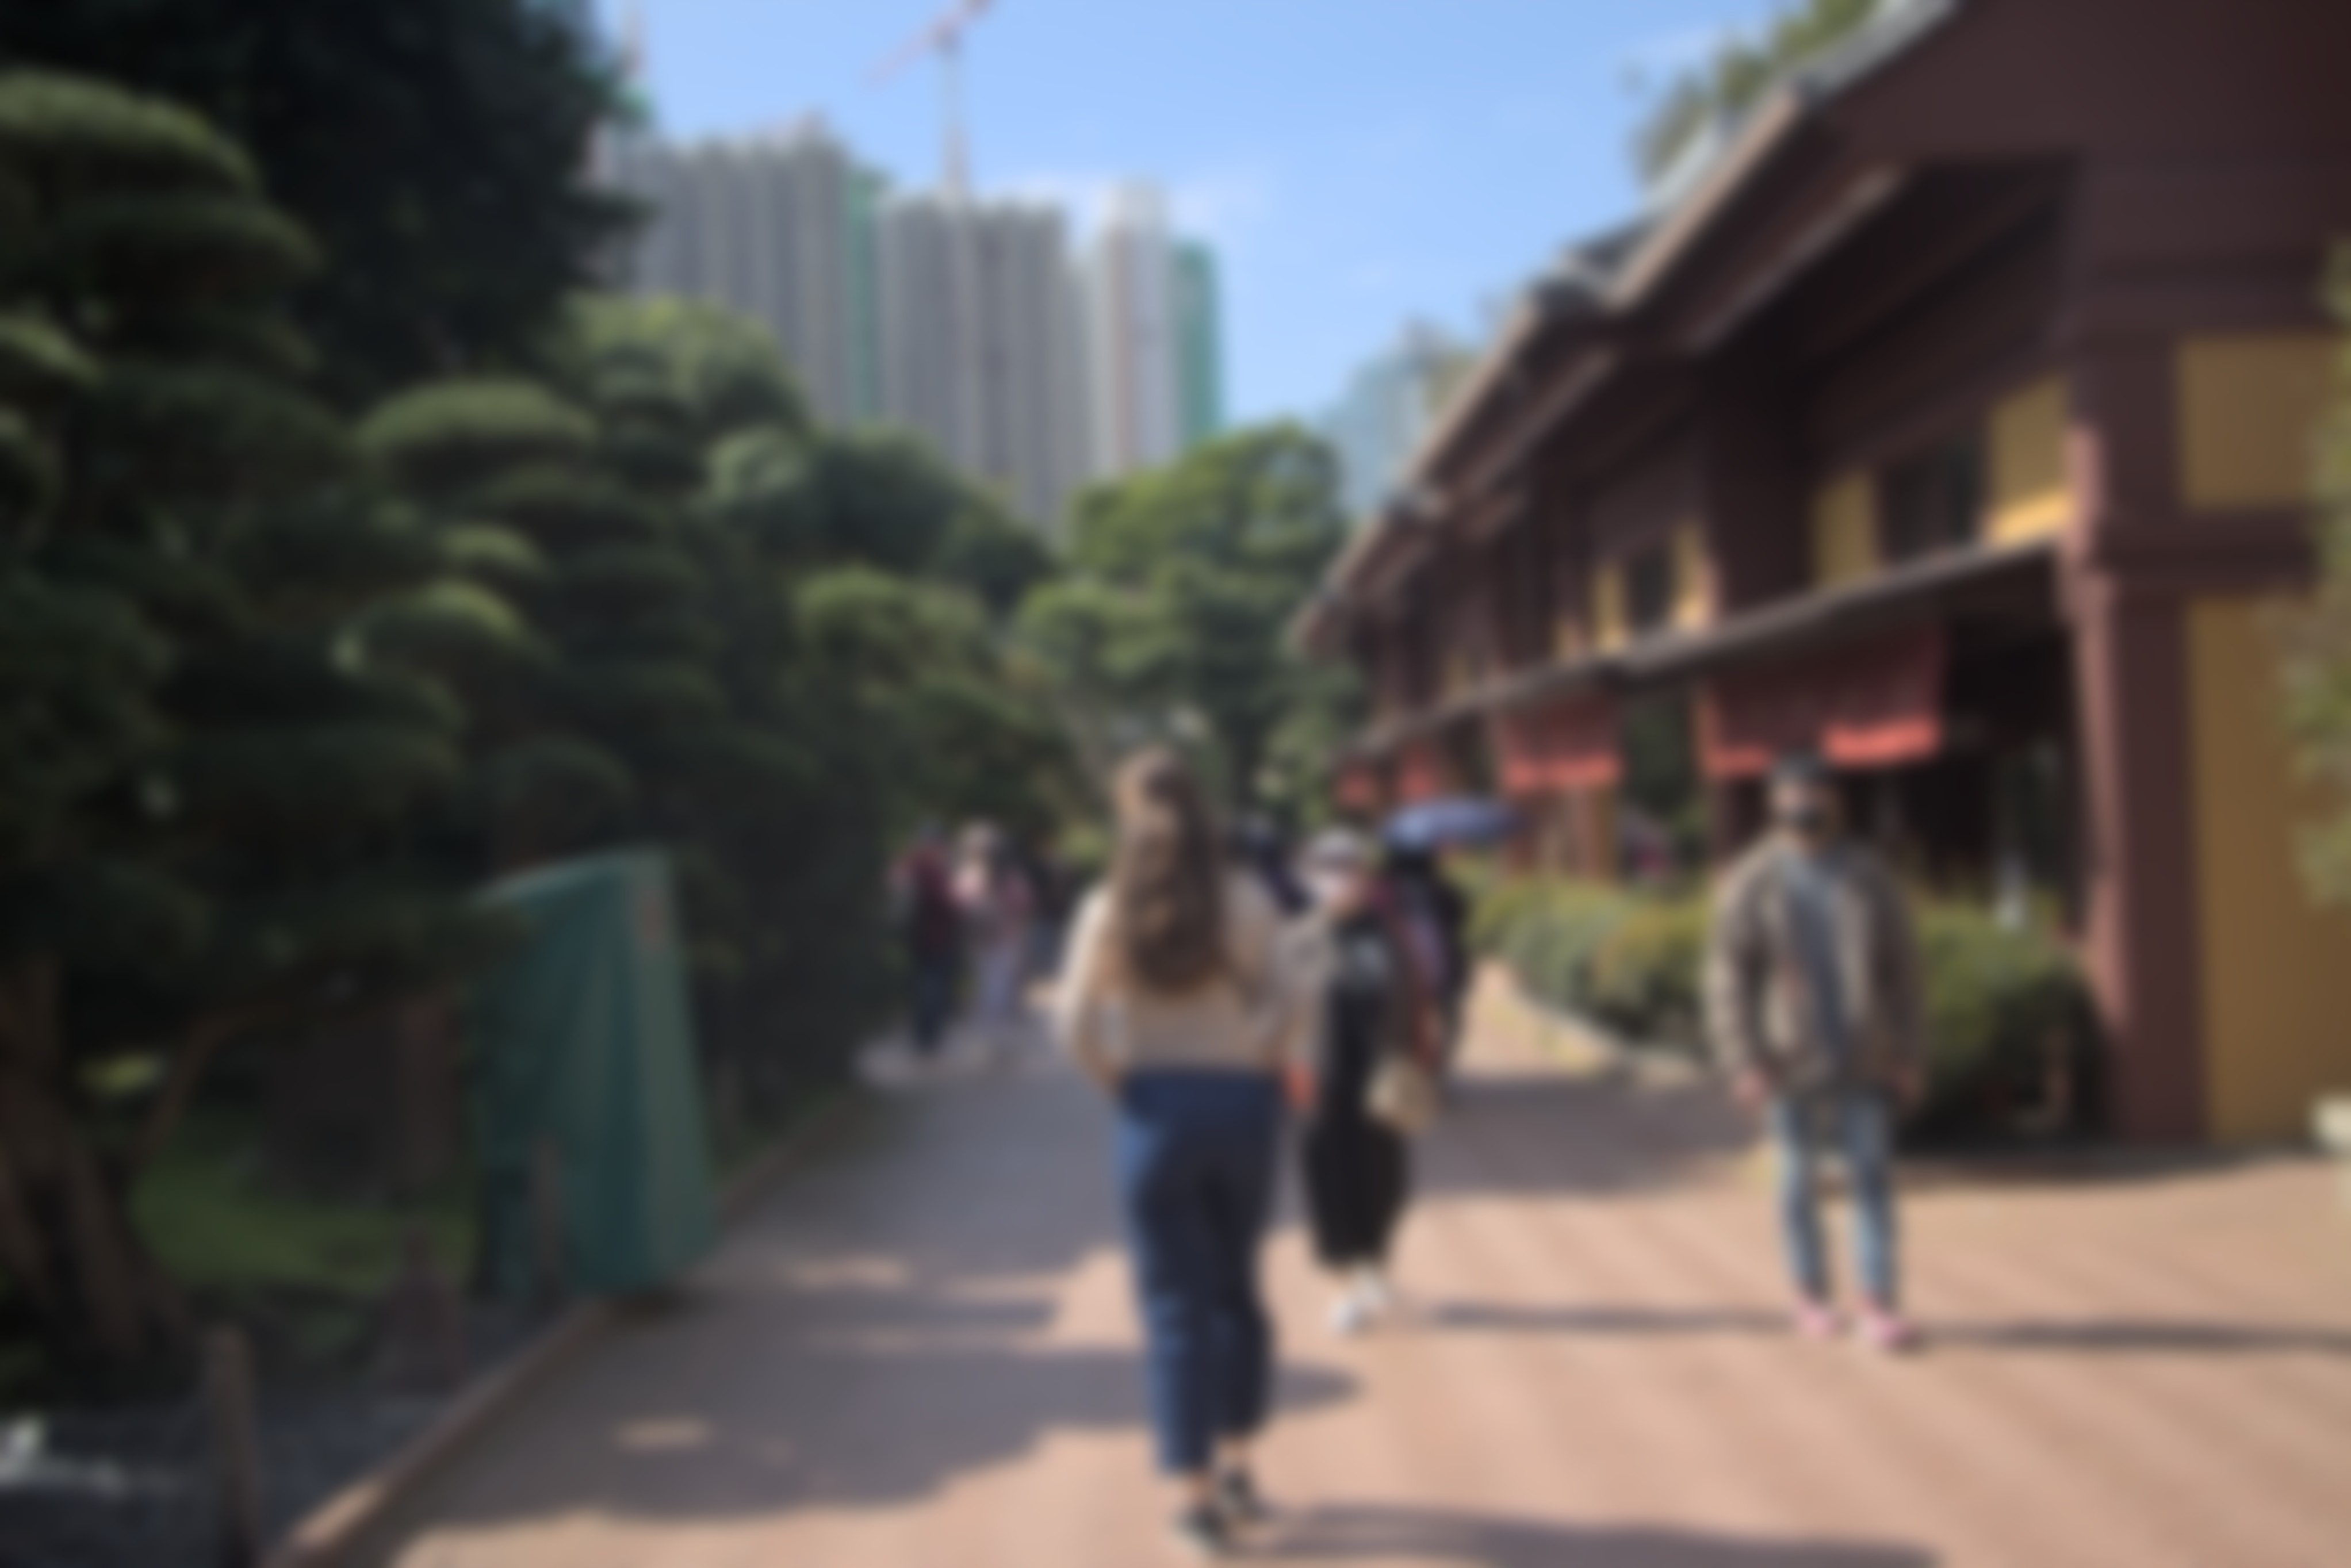
\includegraphics[width=\textwidth]{Images/Obfuscation/blurred_street.jpg}
        \caption{Blurred entire image of Hong Kong street to protect privacy of citizens.}
    \end{subfigure}
    \hfill
    \begin{subfigure}{0.46\textwidth}
        \centering
        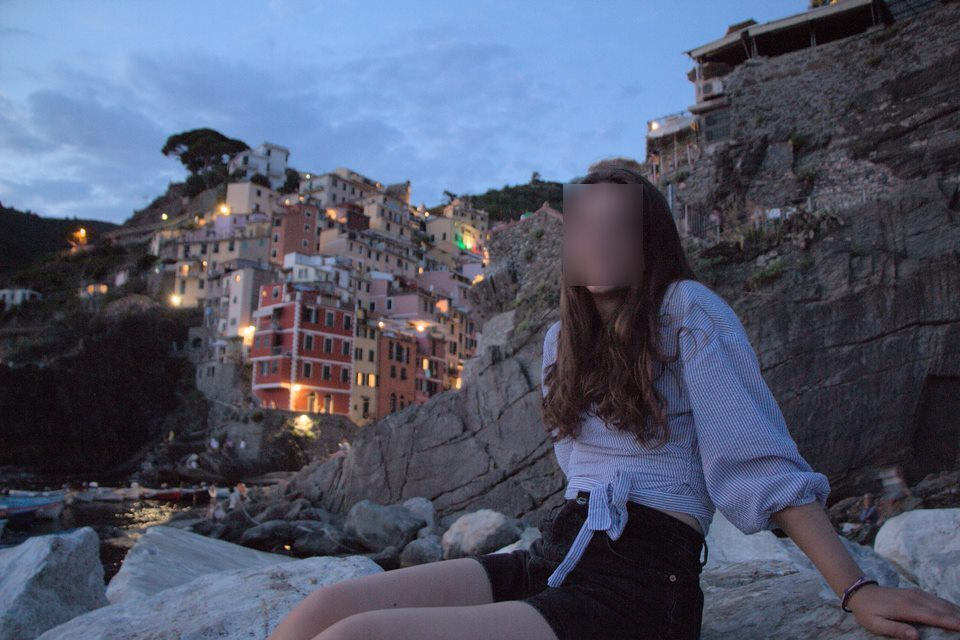
\includegraphics[width=1\textwidth]{Images/Obfuscation/face_blur.jpg}
        \caption{Blurred face of individual by a sea town in Cinque Terre.}
    \end{subfigure}
    \newline

    \begin{subfigure}{0.46\textwidth}
        \centering
        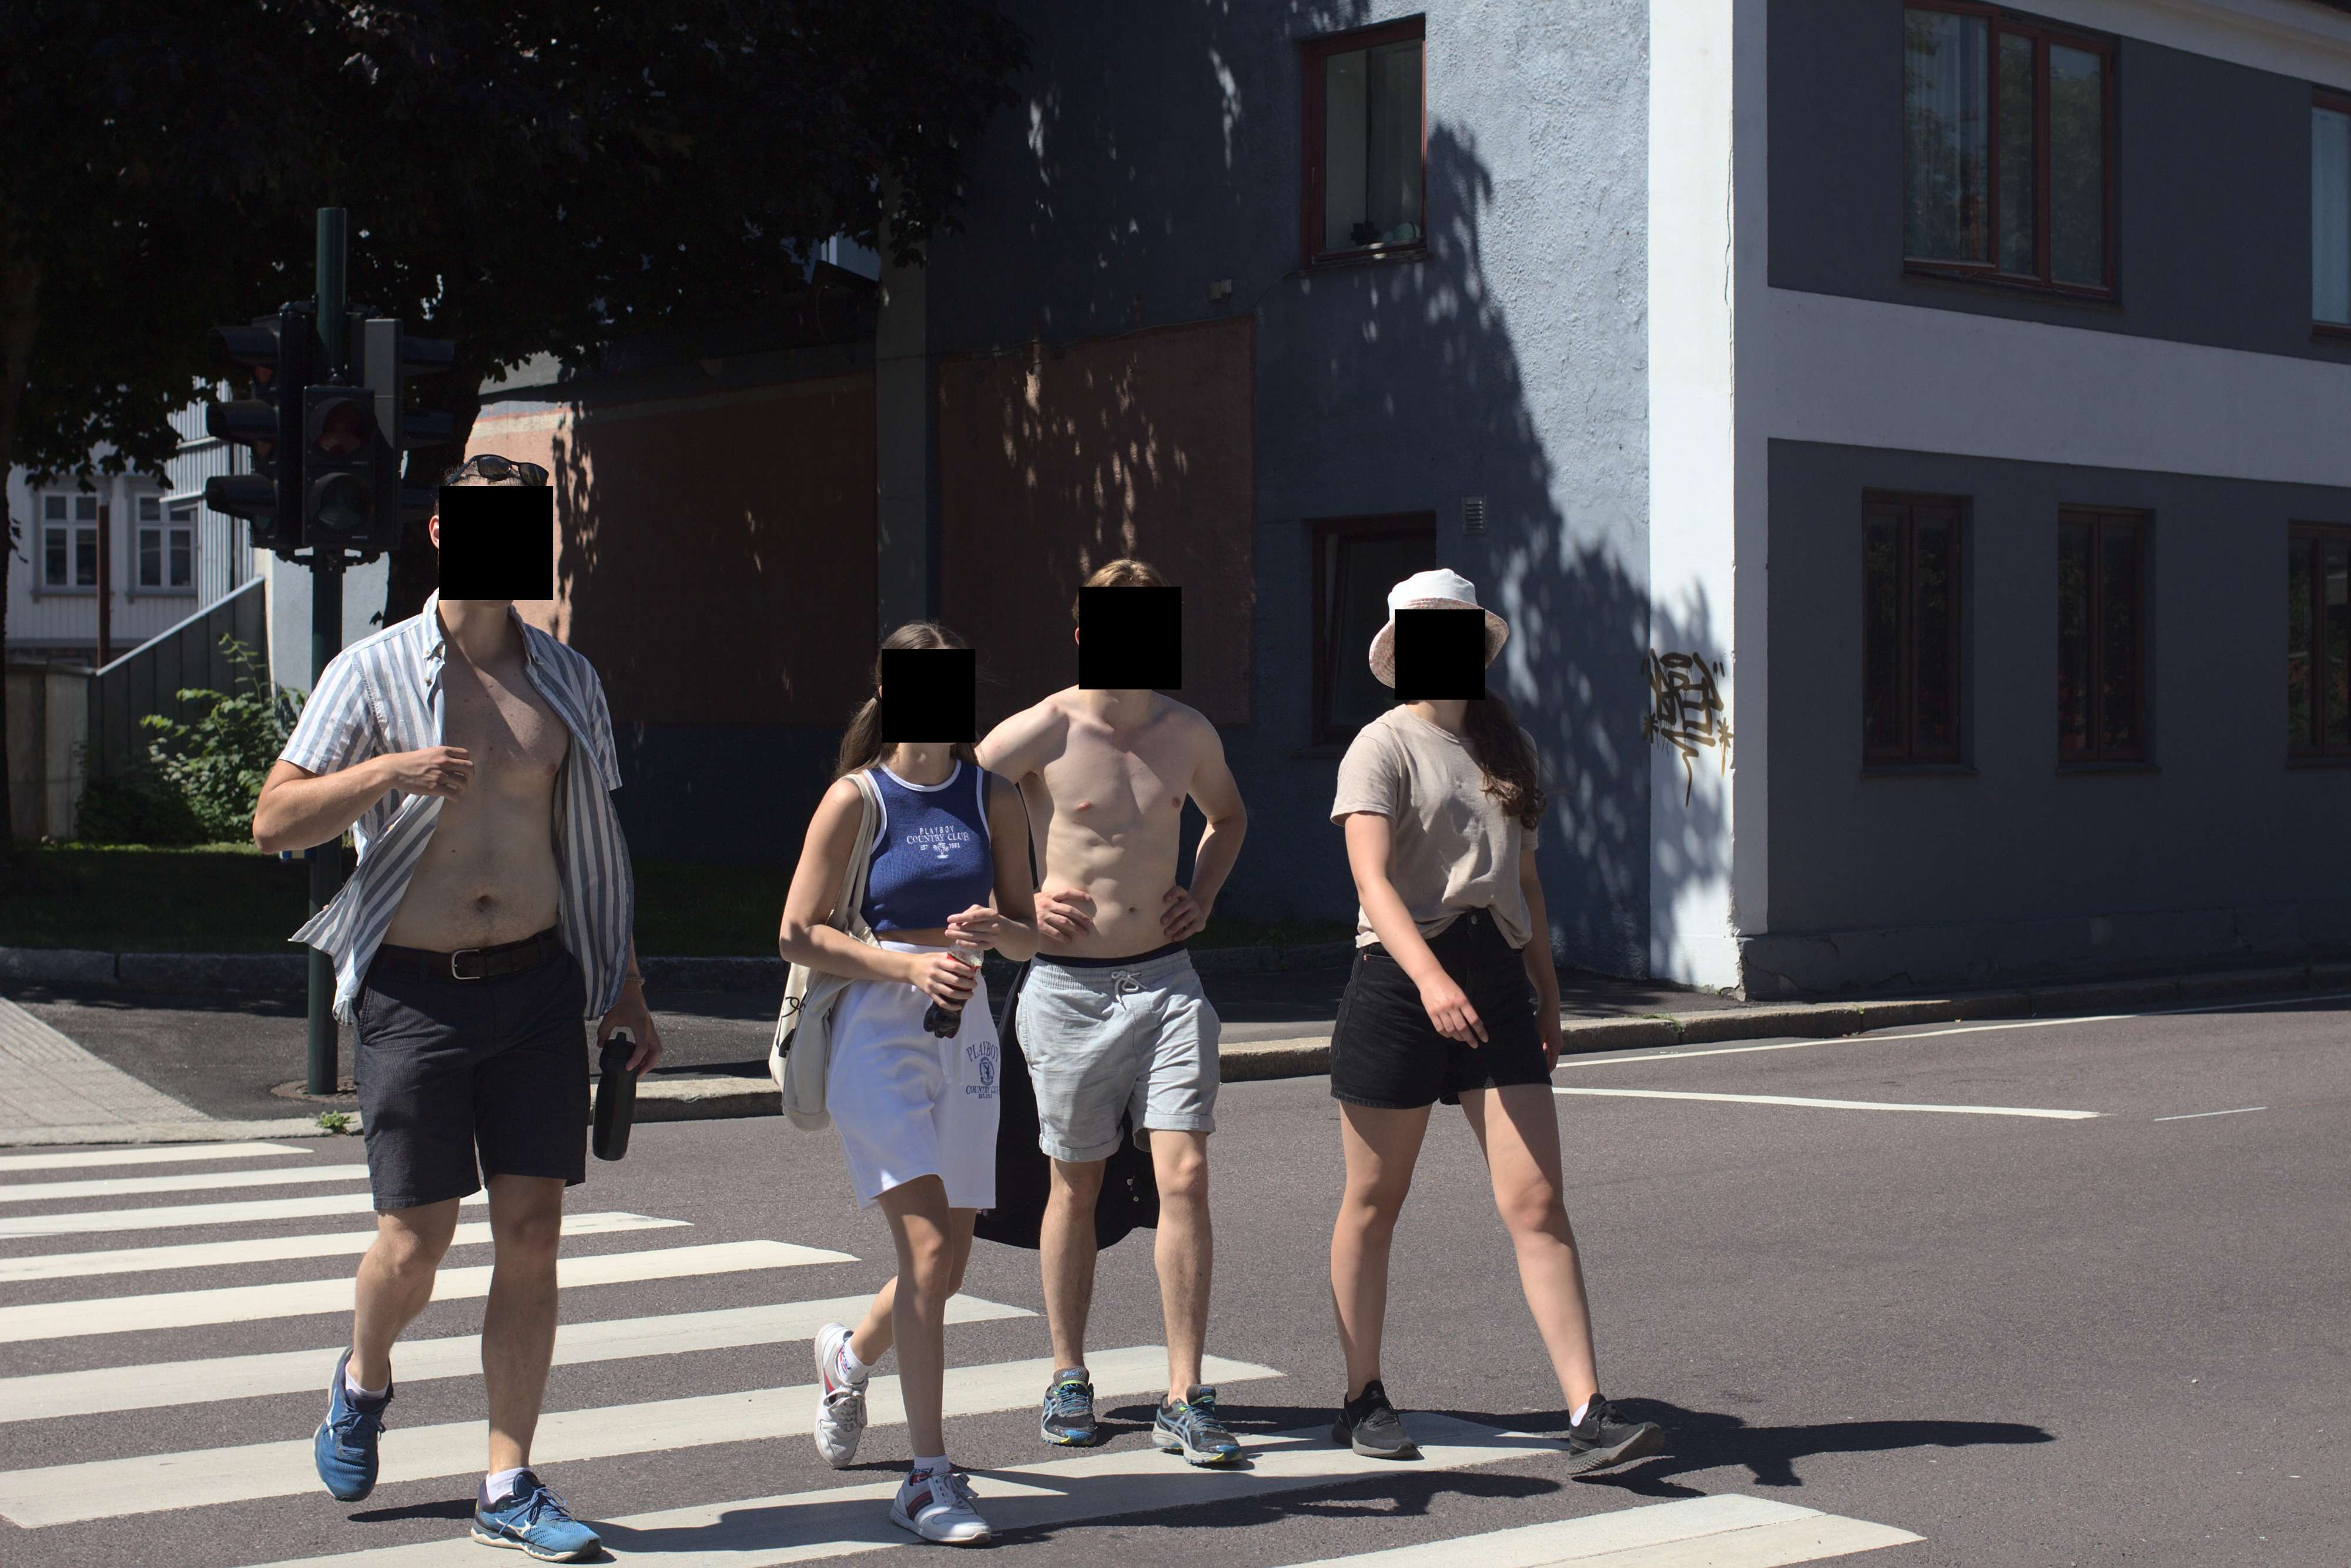
\includegraphics[width=\textwidth]{Images/Obfuscation/tonsberg_gang_masked.jpg}
        \caption{Masked faces.}
    \end{subfigure}
    \hfill
    \begin{subfigure}{0.46\textwidth}
        \centering
        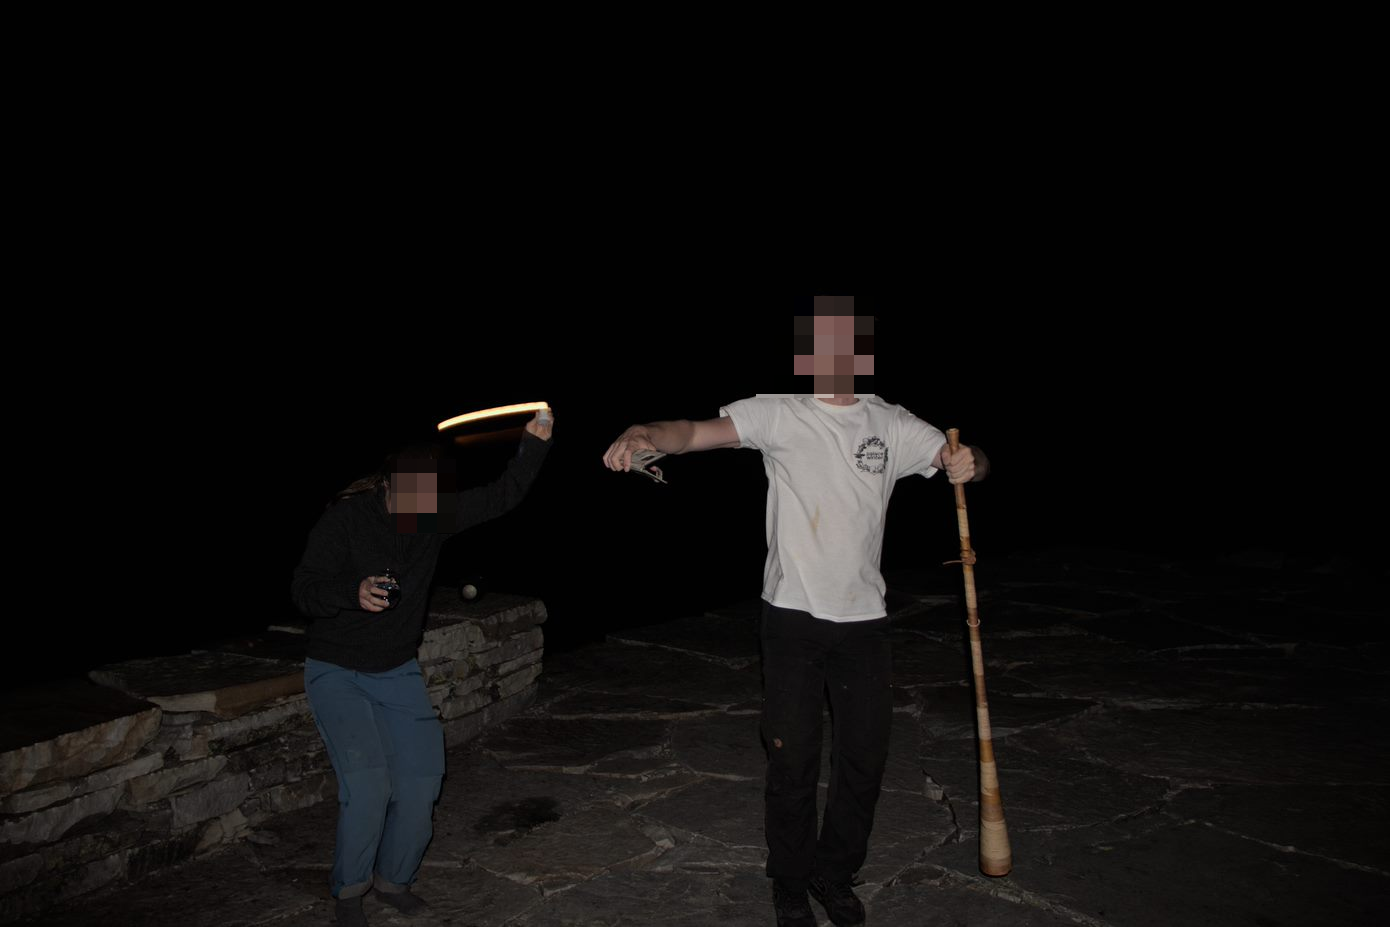
\includegraphics[width=\textwidth]{Images/Obfuscation/gausta_pixelated.png}
        \caption{Pixelated faces.}
    \end{subfigure}
    \newline

    \begin{subfigure}{0.46\textwidth}
        \centering
        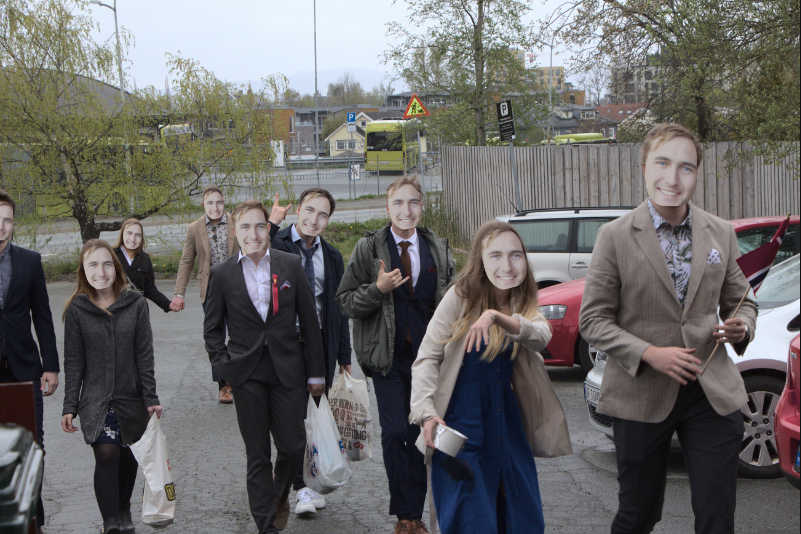
\includegraphics[width=\textwidth]{Images/Obfuscation/me_my_friends_and_I.png}
        \caption{Unconventional method: replace faces. May be done as effectively as the other approaches, but is likely to be seen as an unprofesional approach.}
    \end{subfigure}
    \hfill
    \begin{subfigure}{0.46\textwidth}
        \centering
        
\includegraphics[width=\textwidth]{Images/Obfuscation/white.png}
        \caption{Delete the image. This is the most effective and secure, but removes the possibility of verifying results and is unsuitable for most vision-based applications.}
    \end{subfigure}

    \caption{Six methods to enhance individual privacy in images}
    \label{fig:obfuscation_methods}
\end{figure}

There's also been much research with regards to preserving privacy in the context of machine learning (\cite{ra2023visual_privacy_techniques}). Common to all use cases is the principle that deleting the data is the most definitive method of ensuring privacy, provided that such an action is feasible. When only non-personal data remains stored, the application is unequivocally secure in terms of privacy.

In addition to not protecting the identity of individuals, it is often important that the individuals \textit{feel} their privacy is being preserved.

\subsubsection{User perceptions of smart home IoT privacy}
\label{sec:smarthomeprivacy}

In a 2018 study, researchers conducted semi-structured interviews of 11 smart home owners were conducted to figure out user perceptions of smart home IoT privacy (\citeauthor{zh2018userperceptionsofIoTPrivacy}). What the researchers found, shows promise to IoT edge computing visual devices; the convenience and connectedness of the devices surpasses the desire to preserve privacy. Another research question of the study was user perceptions of obsolescence of the IoT devices, as there are frequent upgrades and new products on the market.

\begin{myquote}{Responses regarding privacy and obsoleteness of IoT devices (\cite{zh2018userperceptionsofIoTPrivacy})}
    "I think it’s more likely that a lot of these things will become obsolete... If that’s what happens then I have to buy another device. It still might be worth it for the convenience" (Participant 10).

    "[The security concern] is always kind of in the back of my mind because of all that IoT stuff that always goes on, and everyone says how easily hackable they are. But I think my peace of mind that I get from having them outweighs my worry of what could be potentially taken advantage of" (Participant 6).
\end{myquote}

\subsubsection{Federated learning}
\label{sec:federated_learning}
In many systems relying on machine learning, being able to utilize locally stored personal data may augment the system to perform better for the situation it was created for. However, sharing this personal data with a centralized model may not be possible due to the legal bases for processing personal data (see sec:legal-bases-processing-personal-data).

\begin{wrapfigure}{r}{0.5\textwidth}
    \centering
    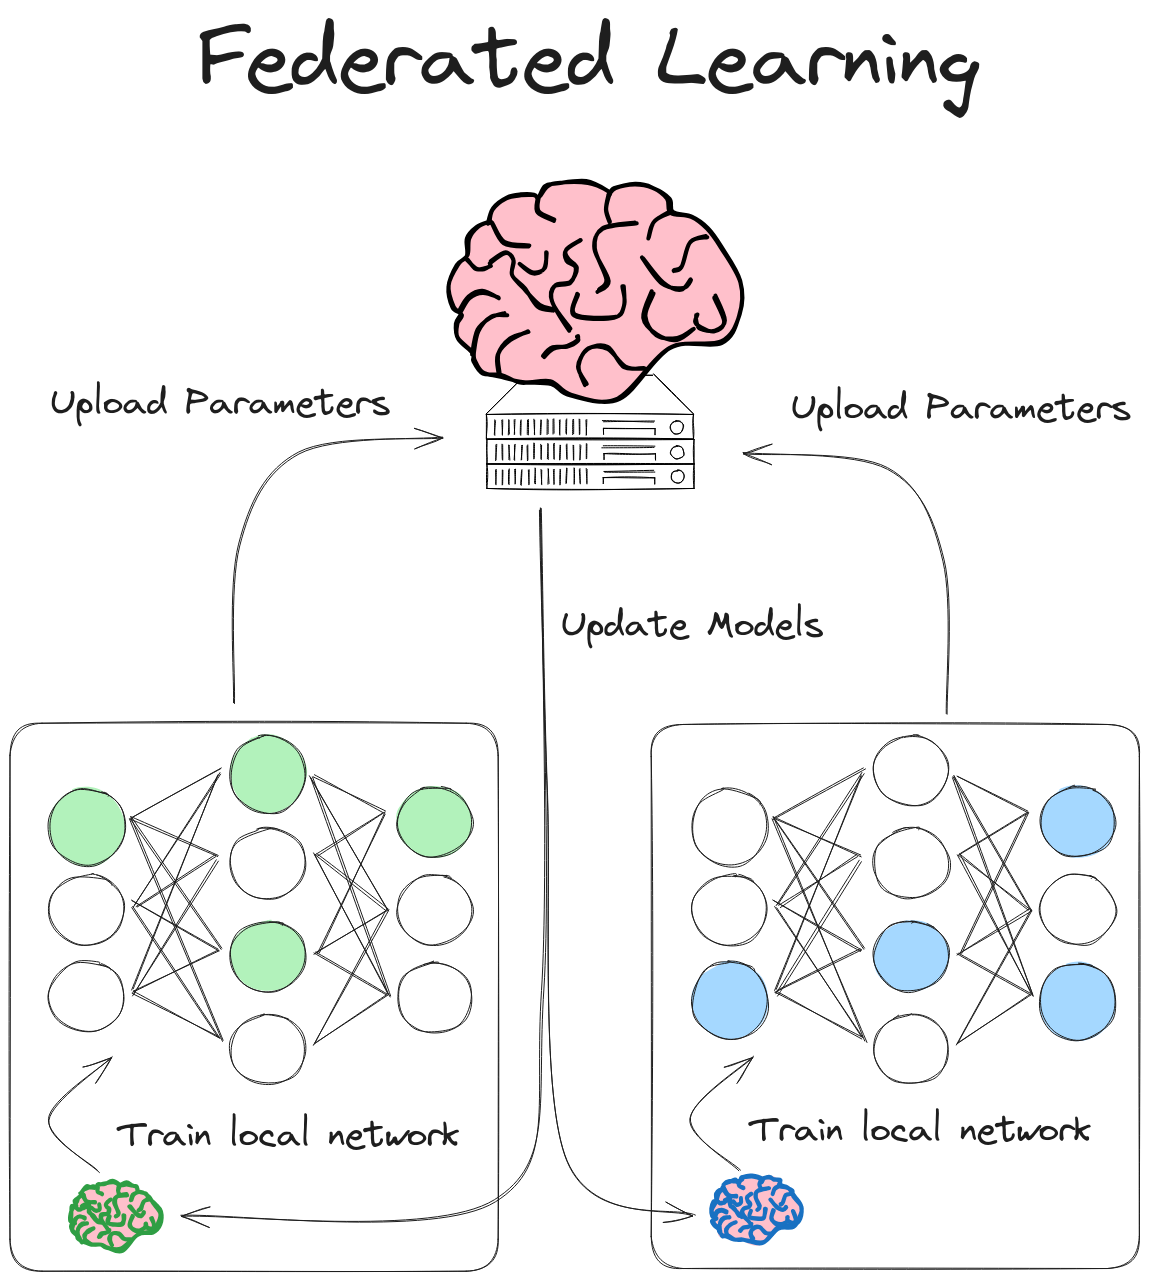
\includegraphics[width=0.48\textwidth]{Images/Diagrams/FL_updated.png}
    \caption{The federated learning process}
    \label{fig:federatedlearning}

    Federated learning (FL), also known as collaborative learning, is a decentralized approach to training machine learning models. It doesn't require an exchange of data from client devices to global servers.
\end{wrapfigure}

The concept of FL can be seen in figure \ref{fig:federatedlearning}, and is best described in the article of \citeauthor{an2022federatedlearninghealthcare} (\citeyear{an2022federatedlearninghealthcare}): "In summary, FL enables the training of ML models locally (at the location of the data) and only shares the resulting model, which is not reverse-engineerable, with the requesting party. Therefore, FL avoids the need to share the private datasets and sensitive data to others, preventing exposition to entities conducting studies and enabling data usage for broader purposes (\cite{re2021servertoclientml}). A central entity manages the learning process and distributes the training algorithm to each participating data holder. Each participant generates a local model trained with their private data and shares the resulting parameters with the central entity. Finally, the central entity employs an aggregation algorithm to combine the parameters of all local models into a single global model".


The FL process is reliant on having ground truth data on the edge for training the models correctly, but obtaining the ground truth for edge device models operating on \textit{visual data} is difficult. The way this may be achieved, is by having a powerful edge device perform the inferences with a computationally expensive but accurate model, and using the inference results of this model as the ground truth for training a separate, possibly faster and less computationally expensive model to replace the other at a later stage. Otherwise, one could also perform the training under conditions where the ground truth is known, for example by manually inputting the number of people in an area, then having the model learn to arrive at the same count based on the camera input.

Improvement of machine learning models devices in the healthcare industry present challenges due to the sensitive nature of medical data from patients. Centralized training of machine learning models may violate laws such as the GDPR, because of the way data is being collected and used unbeknownst to the data subject (\cite{an2022federatedlearninghealthcare}). To tackle these issues, \citeauthor{an2022federatedlearninghealthcare} (\citeyear{an2022federatedlearninghealthcare}) proposes the usage of FL\footnote{Specifically, the FL method described in the works of \citeauthor{ya2019federatedMLconcepts}(\citeyear{ya2019federatedMLconcepts})} to tackle these issues.

Furthermore it should be noted that FL is a method to deal with the existential nature of data in edge computing devices, best described as "isolated islands", and to use the data on edge devices before it is deleted or obscured, to improve the intelligence of the devices in privacy preservant and protective way. An important measure to take in the development of FL models is to ensure that the models are not reverse-engineerable, as the models may contain personal data. This is done by adding noise to the data, which makes it impossible to backtrack the data to the individuals. This may be done by a method such as differential privacy, which is discussed in section \ref{sec:differential-privacy}.

\subsubsection{Differential privacy}
\label{sec:differential-privacy}
The concept of differential privacy is to make data of individuals privacy-preservant through describing them as a group. Data from the group of people may be used, but without the possibility of backtracking the information to certain individuals. See figure \ref{fig:differential-privacy}.

In more technical terms: Differential privacy is a statistical disclosure control algorithm to process individual data from a group to produce close-to-real outcomes without disclosing the personal data of individuals (\cite{hu2023metaverse-privacy}). This means that the data is processed in a way that the results are close to the real results, but the data is not disclosed. This is done by adding noise to the data, which makes it impossible to backtrack the data to the individuals.

Differential privacy is particularly pertinent in the context of federated learning. In this approach, client devices add controlled noise to their model updates—or weights—before sending them to a centralized server. This noise addition prevents the server from being able to infer individual-specific information from the model updates. The degree of noise is regulated by a privacy parameter, often referred to as a privacy budget. This strategy allows the central server to aggregate these noisy updates from all participating nodes to update the global model. Contrary to the original statement, the noise is not removed but rather managed in such a way that the aggregated model maintains utility while protecting individual privacy (\cite{sh2023RolwOfWeightTransmissionProtocolinML})."

Note that differential privacy is a definition, not an algorithm (\cite{dw2011DifferentialP}). In other words, we can have many different algorithms that satisfy the privacy demands for a given use case. For example, \citeauthor{dw2011DifferentialP} mentions the Laplace mechanism (outlined in the same authors works from \citeyear{dw2006noise2sensitivity-laplace}) as an optimal mechanism for answering “tally” type questions differentially privately (\citeyear{dw2011DifferentialP}). For more advanced situations, other algorithms, such as the method outlined by \citeauthor{bl2011learning-privacy} (\citeyear{bl2011learning-privacy}), are more suitable (\cite{dw2011DifferentialP}).

The big tech giants like Apple, Google and Microsoft employ differential privacy in their data collection and analysis to ensure the privacy of their users. Differential privacy is a method to ensure that the data is not personal, and thus not subject to the GDPR.

\begin{figure}[H]
    \centering
    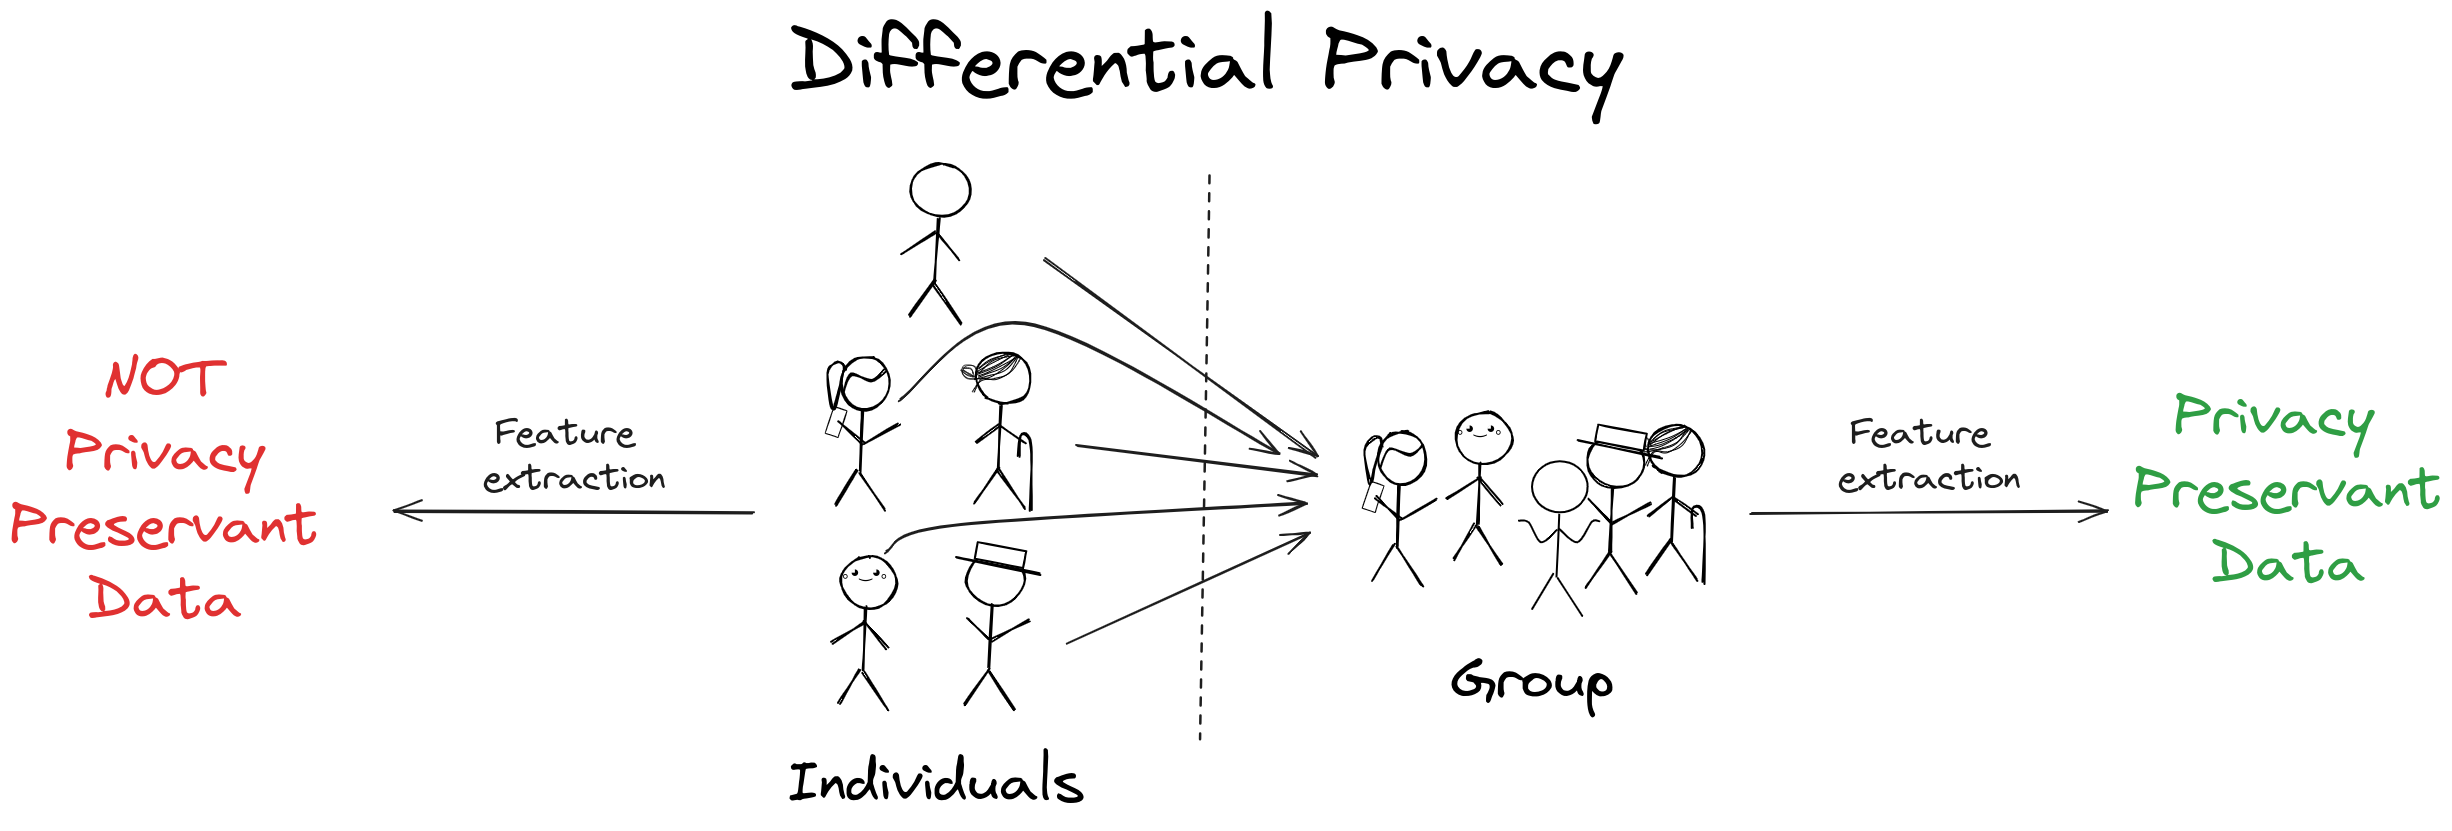
\includegraphics[width=\linewidth]{Images/Diagrams/differential-privacy.png}
    \caption{The differential privacy concept}
    \label{fig:differential-privacy}
\end{figure}

\subsubsection{On-device processing}
According to \citeauthor{hu2022accurateobjectdetectionatedge} (\citeyear{hu2022accurateobjectdetectionatedge}), there are four methods for running tasks on resource-constrained edge computing devices. This is relevant in applications where user's concerns for privacy increases if data is directly transmitted to a server. These methods are seen in table \ref{tab:methods_to_run_tasks}, and explained discussed in the following paragraphs.

\begin{table}[H]
    \centering
    \renewcommand{\arraystretch}{1.5} % Increase vertical padding
    \setlength{\tabcolsep}{1em}
    \begin{tabular}{|l|l|l|}
        \hline
        \rowcolor{gray!25}
        \textbf{Method} & \textbf{Advantages}                & \textbf{Disadvantages}  \\ \hline
        Data encryption & Privacy protection                 & Much bandwidth          \\
                        & Fast calculation                   &                         \\ \hline
        Traditional ML  & Little resource consumption        & Relying on the Internet \\
                        &                                    & Poor robustness         \\ \hline
        Task sharing    & Reducing stress on a single device & Much bandwidth          \\
                        &                                    & Large latency           \\ \hline
        Deep learning   & Privacy protection                 & High resource           \\
                        & High robustness                    & consumption             \\ \hline
    \end{tabular}
    \caption{\centering Comparison of methods for running tasks on resource-constrained
        edge computing devices (\cite{hu2022accurateobjectdetectionatedge})}
    \label{tab:methods_to_run_tasks}
\end{table}

\paragraph{Data encryption}
The first method, data encryption, would be one way of transmitting images in a more secure way. This must be done in a losses way to maintain the image quality to preserve the accuracy of the detectors. Doing so is not trivial, and is a research field on it's own. A few methods are discussed in section \ref{sec:post_analysis_operations}.

\paragraph{Traditional machine learning}
The second method of running traditional machine learning methods, might not the greatest solution either, as they have been less accurate than the deep learning models (see figure \ref{fig:object_detect_20_years}). They may, however, be a good option for devices with low computing power and memory resources as they are generally low-demanding. The methods need less data, are more transparent, but are most applicable to use cases with clear, deterministic logic. Traditional machine learning methods were the most prominent prior to 2014, while deep learning based detection models have been the completely dominant approach to image recognition tasks. Figure \ref{fig:road_map} illustrates a road map of what have been the most popular machine learning approaches to object detection. To achieve similar accuracies to those of the deep learning models but with the low computational demands of traditional machine learning, one might consider to investigate the field of tinyML, discussed in section \ref{sec:tiny_ml_and_frugal_devices}.

\begin{figure}[H]
    \centering
    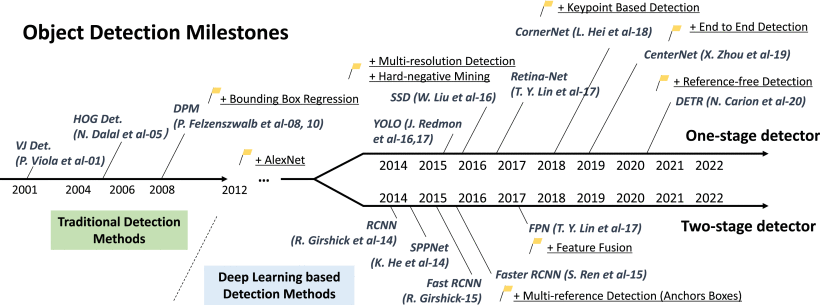
\includegraphics[width=1\linewidth]{Images/Diagrams/object_detection_directions.png}
    \caption{The evolution of object detection (\cite{zou2023object_detection_in_20_years})}
    \label{fig:road_map}
\end{figure}

\paragraph{Task sharing}
The third method, sharing the workload over multiple devices, is not an uncommon practice in technology. See for example Eufy's solution with a "home-base" device in section \ref{par:eufycam}), where camera devices take images and send them to a more powerful computer for doing the heavy computing. This reserves privacy as the images are never sent outside of the local network, and can be achieved by simple TCP/IP\footnote{Transmission Control Protocol/Internet Protocol is a set of standardized rules that allow devices to communicate with each other on a network.} communication between the nodes. This gives low latency, fast networks, but introduces (1) the need of having a central hub, (2) extra work of setting up the transmission protocols, (3) another source of error and (4) the need to encrypt/decrypt images prior/post transmission to ensure security. However, due to scarcity in specialized hardware such as the GPU, this could be a nice solution, as one GPU per facility may be sufficient and achieve a higher throughput than processing large data on the CPUs of multiple edge devices.

\paragraph{Deep learning}
As opposed to traditional machine learning,
This section outlines some methods to retain the privacy of individuals by using different sensors or implementing neural network on the edge devices, often referred to as on-device processing or edge computation. Which term of on-device processing and edge computation is used may be dependent on which aspect of the concept the author chooses to emphasize; the actual process that is happening on a device, or the architectural decision of making the computation on the edge.

\subsubsection{Depth cameras}
A widely used approach within the domain of anonymous fall detection, is to use of RGB depth cameras to capture depth information (\cite{wa2020elderly_fall_detection_meta}). As only depth information is captured, the data remains completely anonymous from the start.

\subsubsection{Deletion of images}
The deployment of visual systems in public spaces presents challenges related to privacy, not only because of the immediate access to private data, but also due to the recent breakthroughs in object detection allowing the extraction of sensitive information from visual data. The altogether only completely safe way to ensure complete and total privacy of data, is to not have the data at all. This may be achieved by the following approach called edge computing.

Edge computing is to have the visual device perform the analysis directly on the device (so called 'on-device processing'). With this approach, the image is obscured or deleted right after analysis without ever leaving the edge device, and only the anonymous analysis results are communicated online. This would mean that the personal data (1) exists \textit{just} while the analysis is running, (2) is never sent online, and (3) is thus a lot less vulnerable to attacks. The perpetrator's device would need to be physically connected to the device and the attack would need to happen in real time. In those cases, the perpetrator could quite likely just as well take the photo himself.

The images would in some cases benefit in multiple ways from being heavily obscured instead of deleted. This approach is discussed in the following paragraph.

\subsubsection{Obfuscation}
\label{sec:obfuscation}
Another way to remove the privacy concern is by obscuring the images after analysis in such a way that individuals may never be identified.

Obfuscation is the action of making something obscure, which means to conceal or make unclear, implying it has been done intentionally. To obscure an image is often used interchangeably with “to blur”, but they are not the same. To blur means to make something indistinct or hazy, suggesting something is unclear or out of focus. One might say an image has been obscured by blurring the image, or it may be done by other methods such as masking or pixelate the faces of individuals. These methods are illustrated in figure \ref{fig:obfuscation_methods}.

\paragraph{Blurring the faces}
In a \citeyear{ma2019fall_anonymous} study, faces were detected with a thermal-detecting camera and then photos were captured with an RGB camera, blurring the area the face was detected by the thermal camera (\citeauthor{ma2019fall_anonymous}). This approach is privacy preservant as long as all faces are blurred, but may fail if the algorithm does not detect all faces. In those cases, however, most humans would likely also struggle to identify a person based on the face. On the contrary, in many cases, blurring the entire image would compress the image, making it faster and easier to transfer, and be the faster option than having to detect all faces in an image.

\paragraph{Perceptions of privacy enhancements methods}
A questionnaire study of 328 students indicated that blurred images were not considered by the students to provide satisfactory privacy protection (\cite{ed2012privacy_review}). Participants were given 18 randomly ordered videos, and were asked to rate the privacy on a Likert\footnote{Likert scale: A scale of odd options, where the participant may answer a neutral middle-option and distribution should be equally distributed in both directions thereafter. An often used questionnaire scale in psychology research.} scale from 1-5. The obfuscation methods, or privacy enhancements as they called them, and the results are displayed in figure \ref{fig:ed_results}. The results show that blurred images were only considered privacy preservant for 23 percent of participants. Regardless, an important notion is that the images of this survey are from within a private home, posing higher demands and expectations with regards to privacy than what is typically done in a more public space.

\begin{figure}[H]
    \centering
    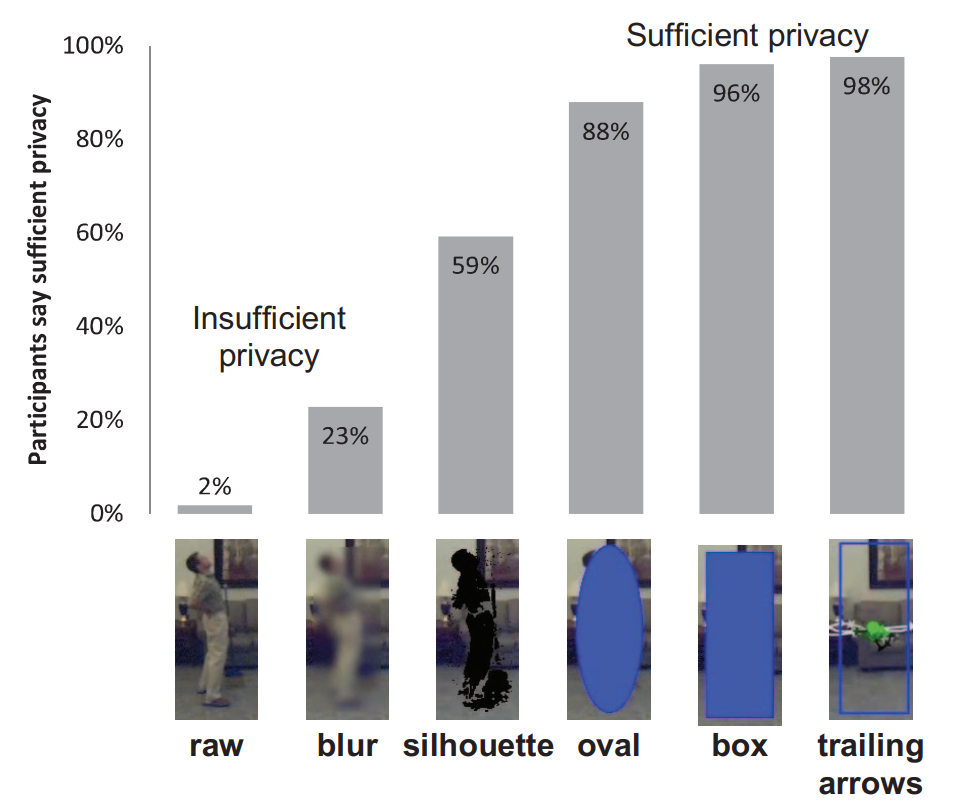
\includegraphics[width=0.6\textwidth]{Images/ed2012results.png}
    \caption{Privacy enhancements methods in the study of  \citeauthor{ed2012privacy_review} (\citeyear{ed2012privacy_review})}
    \RaggedRight The study indicates that the methods of blurring an image is not perceived privacy preservant. However, as we will see in section \ref{sec:deletion_vs_obs_discussion}, the results of this study might not be a reason by itself to throw the method of blurring an image out the window.
    \label{fig:ed_results}
\end{figure}

\subsubsection{Ethical Considerations in the Development of Localization Technologies}
\label{sec:ethics_localization_tech}

As we advance the capabilities of technologies such as YOLOv9 for human localization, it becomes imperative to consider the ethical implications of our developments. The narrative of George Orwell's dystopian novel \textit{1984} serves as a stark reminder of the potential societal consequences of pervasive surveillance and control. Orwell's portrayal of a society where history is constantly rewritten and individual privacy is obliterated highlights the dangerous path we might tread if these technologies are misused.


\begin{wrapfigure}{r}{0.5\textwidth}
    \centering
    
\includegraphics[width=0.48\textwidth]{Images/Ethical/redmon-twutter-stoppedCV.png}
    \caption{Redmon Quit Computer Vision Research Due to Ethical Concerns}
    \label{fig:redmon-twitter-stoppedCV}
\end{wrapfigure}

\paragraph{Historical Precedents and Personal Accountability}
The decision by Joseph Redmon, the creator of the initial versions of YOLO, to cease his work on the project due to its military applications illustrates a profound ethical stance. Redmon's choice underscores the responsibility that developers bear in considering the broader impacts of their work, paralleling Orwell’s caution against allowing technological advances to override ethical judgments. Joseph Redmon's resignation from the development of YOLO due to ethical concerns marks a critical point in the discourse on the moral responsibilities of researchers and developers in the field of artificial intelligence and machine learning. The discussion of AI development is still very much ongoing.

\begin{myquote}{Greed's Grief}
    For the love of money is a root of all kinds of evil. Some people, eager for money, have wandered from the faith and pierced themselves with many griefs. -1 Timothy 6:10, The Bible.
\end{myquote}

\paragraph{Ethical Framework for Development}
In developing technologies capable of tracking and analyzing human behavior, we must establish robust ethical frameworks that prevent misuse and ensure that advancements enhance societal welfare without infringing on individual rights and freedoms. This involves transparent development processes, clear privacy safeguards, and continuous monitoring of technology deployment.

\paragraph{Learning from History}
Just as Orwell warns against the dangers of forgetting or altering history, the AI community must remember the lessons from pioneers like Redmon. We must strive to develop technologies that do not compromise ethical standards for convenience or profitability.

\paragraph{Conclusion}
The development of localization technologies presents complex ethical challenges that require us to be vigilant and proactive. By embedding ethical considerations into the fabric of our technological innovations, we can avoid the dystopian futures forewarned by Orwell and ensure that these tools serve to support and enhance human society, rather than diminish it.

\subsection{Object Detection}
This subsection includes a brief summarization of the evolution of object detection, including the transition from traditional methods to morw modern methods such as the YOLO series and vision transformers.

The evolution of object detection can be divided into two major historical phases: before and after 2014, as illustrated in Figure \ref{fig:object_detect_20_years}. Prior to 2014, traditional object detection methods, such as the Viola-Jones detectors (\cite{vi2001viola-jones-orig}), Histogram of Oriented Gradients (HOG), and Deformable Part-Based Models (DPMs) were prevalent\footnote{These are just some honorable mentiones of some of the most sucessful and widely adopted models of the time (\cite{li2012violajonessuccessful})}. During this era, "mixture models" were developed to improve detection granularity by recognizing the different parts of the same object, such as the doors and windows of a car.

Despite these advancements, it was not until the introduction of Region-based Convolutional Neural Networks (R-CNN) in 2014 that the accuracy of object detection systems began to improve significantly. This paradigm shift marked a substantial advancement in the field, leveraging deep learning techniques to enhance detection performance dramatically (\cite{zou2023object_detection_in_20_years}). The period following 2014 has seen rapid progress, introducing sophisticated object detectors like You Only Look Once (YOLO) and Detection Transformers (DETR). These are explored in greater detail in section \ref{sec:rtdetr} and \ref{sec:yolov9}

Machine learning can be seen as a gamified\footnote{apply typical elements of game playing (e.g. point scoring, competition with others, rules of play) to (an activity), typically as an online marketing technique to encourage engagement with a product or service. (\cite{ox2023gamification})} version of statistics and software engineering. Object detection is a subset of machine learning. Modifications and new advances in object detection methods may be instantly evaluated by running inference on benchmark datasets and compare them to the other state of the art (SOTA) models.

\subsubsection{Performance benchmark}
\label{sec:performance_benchmark}

\paragraph{Dataset}
There are multiple benchmark datasets for machine learning applications. The area of facial emotion recognition alone has at least five benchmark datasets (\cite{sa2022facialemotions}). For the task of object detection, the Common Objects in Context (COCO) dataset (\cite{li2014cocodataset}) has been widely used since it's introduction in 2014, with it's 330 000 annotated images.

Another well-known, widely adopted dataset for classification, object detection and segmentation is the PASCAL Visual Object Classes (VOC) (\cite{ev2010pascaldataset}). The PASCAL VOC websites include several challenges, i.e. VOC2005 through VOC2012, for researchers to benchmark their detectors. Even though the challenges have completed, one can still evaluate new methods on their datasets.

A third dataset is the CrowdHuman dataset. This may be the most relevant for a detector aiming to detect persons, as it consists of 24 370 images with in total 400 000 human instances in diverse occlusions and variations.

For any use case implementation however, it is vital to have a dataset that is relevant to the problem at hand. For a detector aiming to detect persons in a dark-lit museum, the most relevant dataset would be one with images from dark-lit museums.

In real-world applications there are licenses for using datasets for training a model. Testing and benchmarking a solution against a certain dataset is typically free to do, but the datasets are often under a license which forbids commercial use.

\paragraph{Accuracy of Model Inferences}
\phantomsection
\label{sec:accuracy_of_model_inferences}
Due to the aforementioned gamified nature of machine learning models, which metrics are deemed important may have a significant impact on the development of the models. According to \citeauthor{zou2023object_detection_in_20_years}, these developments primarily pursue two main goals: enhancing prediction accuracy and increasing computational efficiency (\citeyear{zou2023object_detection_in_20_years}. Additionally, the evaluation of object detectors extends to more, harder-to-measure, abilities. This can be their ability to transfer their capabilities to new domains, such as learning to detect a new category it has not previously been trained for.

However, the most used measurement of performance for an object detector model is the \textit{mean Average Precision} (mAP) for varying values of \textit{IoU thresholds} (\cite{zou2023object_detection_in_20_years}). 

The average precision is the average when taking the sum of precision values under various recalls. The mean is when this is averaged for all the object classes in the dataset. The IoU brings bounding box positioning into the equation, representing how well the predicted box fits to the ground truth. A detailed explanation of what this means is given in the following paragraphs.

First we need to understand the concepts of true positives, false positives, false negatives, the confusion matrix, precision and recall. These are easiest to explain if the task is image classification and not object detection. For \ref{sec:understandingtp} and \ref{sec:understandingprecision}, we will use the example of image classification, but the concepts are the same for object detection, with the difference that the bounding box positioning is also taken into account.

\paragraph{Understanding TP, FN, and FP, and the Confusion Matrix}
\phantomsection
\label{sec:understandingtp}
For a machine learning model dealing with a regression problem\footnote{Object detection is also a regression problem, as the model is simply relating the independent variable input image pixels to a dependent variable output of the bounding boxes and classes.}, the metrics usually used to evaluate it's performance is the number of true positives, false negatives and false positives. 

These may be defined as follows:
\begin{enumerate}
    \item True Positive (TP): The number of instances correctly identified by the model as positive. For instance, if your model is tasked with identifying people in images, a true positive would be an instance where the model correctly identifies a person.
    \item False Negative (FN): The number of instances where the model incorrectly identifies a positive instance as negative. Using the same example, this would be a situation where the model fails to identify a person who is actually in the image.
    \item False Positive (FP): The number of instances where the model incorrectly identifies a negative instance as positive. This could occur if the model identifies a person in an image where there is no person.
\end{enumerate}

The confusion matrix is a table used to illustrate these numbers. An example of a confusion matrix is shown in figure \ref{fig:confusion_matrix}. This model has identified 915 people correctly, failed to identify 128 people, and incorrectly identified 97 instances as people when there were none.

\begin{figure}
    \centering
    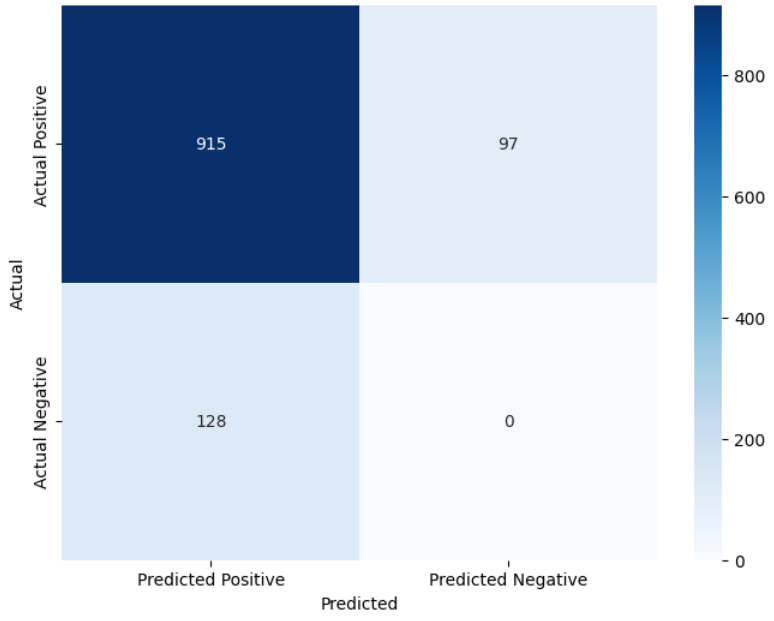
\includegraphics[width=0.5\linewidth]{Images/Diagrams/confusion_matrix.png}
    \caption{An example of a confusion matrix.}
    \label{fig:confusion_matrix}
\end{figure}

Further the TPs, FNs and FPs are used to calculate the precision, recall and F1 score of a machine learning model.

\paragraph{Understanding Precision and Recall}
\phantomsection
\label{sec:understandingprecision}
For a balanced metric of precision and recall we also have the F1 Score, combining the two in a single value. Here’s a breakdown of each:

Precision: Measures the accuracy of positive predictions. It is the ratio of correctly predicted positive observations to the total predicted positives. High precision relates to a low rate of false positives. For object detecion of persons, precision would be how accurate the model is when it claims to detect a person.
\[
\text{Precision} = \frac{TP}{TP + FP}	
\]

Recall (Sensitivity or True Positive Rate): Measures the ability of the model to find all the relevant cases within a dataset. It is the ratio of correctly predicted positive observations to the all observations in actual class. High recall relates to a low rate of false negatives. For object detection of persons, recall would tell us how many of the actual persons in the image the model was able to detect.
\[
text{Recall} = \frac{TP}{TP + FN}	
\]

F1 Score: The weighted average of Precision and Recall. This score takes both false positives and false negatives into account. It is particularly useful when the class distribution is uneven. F1 Score is best if there is some sort of balance between Precision and Recall in the system.
\[
\text{F1 Score} = 2 \times \frac{\text{Precision} \times \text{Recall}}{\text{Precision} + \text{Recall}}
\]

To assess a regular machine learning model's performance, the precision-recall curve is still a common practice. The precision-recall curve is a graph that shows the trade-off between precision and recall for different thresholds for confidence in the object class. As you allow your model to be more uncertain in it's inferences on the image, the number of hallucinations will also increase and thus the precision drops.

todo sett inn precision recall curve

% \begin{figure}[H]
%     \centering
%     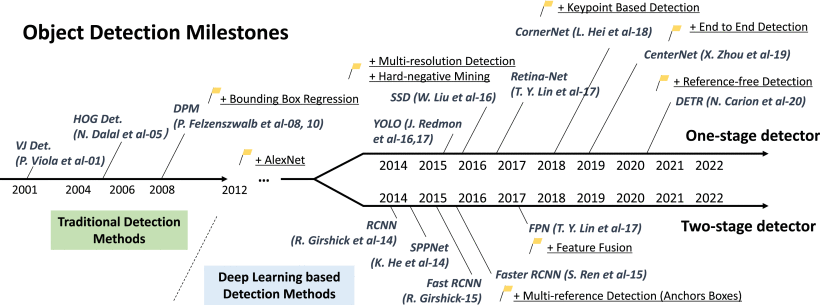
\includegraphics[width=1\linewidth]{Images/Diagrams/object_detection_20years.png}
%     \caption{The evolution of object detection (\cite{zou2023object_detection_in_20_years})}
%     \label{fig:object_detect_20_years}
% \end{figure}

\paragraph{Understanding the IoU metric}

Accuracy in object detection refers to both detecting the object \textit{and} it's location accurately. Combining both in one metric would simplify benchmarking. The precision, recall and f1-score all neglect the positioning precision of bounding boxes. For assessing localization accuracy, the Intersection over Union (IoU) is calculated. This compares the predicted bounding box and the ground truth bounding box in a way so boxes need to fit as closely to the ground truth bounding box as possible to get the best score (which is 1.0). See figure \ref{fig:IoU} for an illustration. The equation is simple:

\[
    \text{Intersect over Union} = \frac{\text{Area of Overlap}}{\text{Area of Union}}
\]

Following the introduction of MS-COCO datasets in 2014, researchers started to pay more attention to the accuracy of object localization. Instead of using a fixed IoU threshold\footnote{A fixed IoU threshold is typically set at 0.5 or higher. Which value is best dependends on the accuracy demands of the sceneario, and is why having the value the ability to adjust the threshold is a good idea when implementing an object detector}, MS-COCO AP is averaged over multiple IoU thresholds between 0.5 and 0.95, which encourages more accurate object detector localizations (\cite{zou2023object_detection_in_20_years}.

\begin{figure}
    \centering
    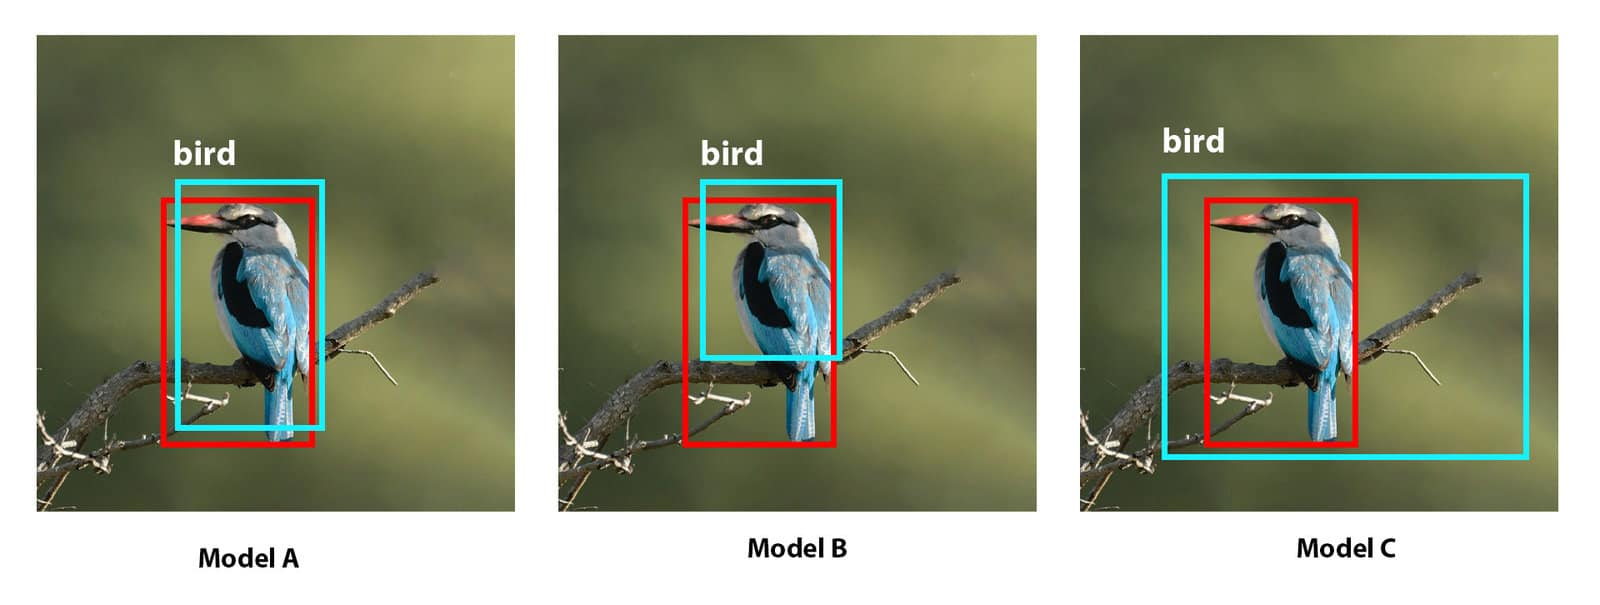
\includegraphics[width=0.5\linewidth]{Images/Diagrams/IoU.jpg}
    \caption{Intersection over Union (IoU) metric}
    \label{fig:IoU}
\end{figure}



% evne til å forbedre mørke scener i mobiltelefonteknologi vil kanskje også over noen år bli overført til mer lavnivåsystemer.
% Primary objective demonstrate feasability and effectiveness of on-device human detection and tracking in a practical and realistic setting.
% Burde være en sekundary goal her kanskje å lage en heatmap.
% Avveie om lysstyrke, bevegelse, bilder, sett fra menneske og maskin er det samme.

\subsubsection{Real-Time Detection Transformer}
\label{sec:rtdetr}
The Real Time Detection Transformer (RT-DETR) is a real-time object detection model developed by the Facebook (Meta) Research team. The model uses a Transformer encoder-decoder architecture similar to a large language model. See figure \ref{fig:detrarchitecture} for an illustration of the architecture.

\begin{figure}
    \centering
    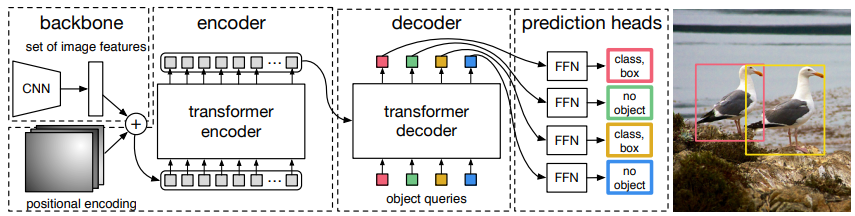
\includegraphics[width=1\linewidth]{Images/Diagrams/DETR2.png}
    \caption{The architecture of the DETR model (\cite{carion2020endtoend}).}
    \label{fig:detrarchitecture}
\end{figure}

In the paper first introducing the model, \citeauthor{carion2020endtoend} claim it outperforms competitive baselines on panoptic segmentation\footnote{This is a challenging pixel-level segmentation task. In segmentation tasks, an image is divided into meaningful regions. Altough different from object detection.} with a simple segmentation head trained on top of a pre-trained DETR. 

The conclusions of the paper are as follows:
"We presented DETR, a new design for object detection systems based on transformers and bipartite matching loss for direct set prediction. The approach achieves comparable results to an optimized Faster R-CNN baseline on the challenging COCO dataset. DETR is straightforward to implement and has a flexible architecture that is easily extensible to panoptic segmentation, with competitive results. In addition, it achieves significantly better performance on large objects than Faster R-CNN, likely thanks to the processing of global information performed by the self-attention. This new design for detectors also comes with new challenges, in particular regarding training,  optimization and performances on small objects. Current detectors required several years of improvements to cope with similar issues, and we expect future work to successfully address them for DETR." (\cite{carion2020endtoend}).

And 

\subsubsection{YOLOv9}
\label{sec:yolov9}
The YOLO (You Only Look Once) object detection algorithm is a popular choice for real-time object detection. YOLO processes images in a single pass, making it faster than traditional object detection algorithms that require multiple passes. YOLO divides the image into a grid and predicts bounding boxes and class probabilities for each grid cell. The YOLOv9 is an improved version of the original YOLO algorithm, incorporating various enhancements to improve detection accuracy and speed. The YOLOv9 model is pre-trained on the COCO dataset. This is previously introduced dataset contains 80 different classes which the model is able to detect. 

\begin{myquote}{YOLOv9 author's comment on the DETR series}
    "However, since it is extremely difficult for DETR series object detector to be applied to new domains without a corresponding domain pre-trained model, the most widely used real-time object detector at present is still YOLO series." (\cite{wa2024yolov9}).
\end{myquote}



\subsubsection{Dark-Lit Environments}
Being able to detect and locate people in dark-lit environments have been previously attempted, usually for security concerns in public spaces. \citeauthor{pa2020PersonDetectionNightTimeFLIR} developed a system for detecting people in dark-lit environments using a convolutional neural network. They modified the three input channels which usually take RGB to take as input instead (i) the original infrared image, (ii) a difference image from the previous frame, and (iii) a background subtraction mask. Their dataset is vastly different from the setting for this thesis, as the individuals in their photos were far away from the cameras. However, they found that their system was able to detect people in dark-lit environments with an accuracy of 90\%. This is a promising result, as it shows that it is possible to detect people in dark-lit environments using infrared imaging and CNNs. They used FLIR cameras, which make images from heat. Doing inferences on pure infrared images may be harder because the infrared radiation may be less prevalent than the heat a FLIR camera may capture. The FLIR cameras are expensive, and thus not considered viable for this project.
\cite{pa2020PersonDetectionNightTimeFLIR}.


todo les YOLO in the Dark - Domain Adaptation Method for Merging Multiple Models

\subsubsection{Effectiveness of Training Dataset Specialization}
\label{sec:dataset_specialization}
Comparison of various algorithms performance enhancement when data has been optimized for the use case. What is the role of a training dataset in the task of determining the weights in a yolov9 artificial neural network, and how can would special training data optimize the weights for a specific use case?

Transfer learning is typically when a trained model is used as a starting point for a new model, and then fine-tuned on a new dataset. This is a useful to extend the trained models capabilities to for example learn how to correctly identify a new object class. In this thesis, the goal is to improve the performance of the YOLOv9 model by training it on a dataset that is specialized for the museum environment. The dataset used for training the YOLOv9 model in this thesis is the COCO dataset, which is a large dataset of images with 80 different classes. The COCO dataset is a general dataset, and the YOLOv9 model trained on this dataset may not perform optimally in the museum environment. By training the YOLOv9 model on datasets that are more similar to the acquarium environment, we will not extend the models capabilities in the same way as what is typically done in transfer learning as we are trying to reduce the number of classes to 1 (person), and we are trying to improve on it's already learnt capability of identifying persons.

\textbf{The datasets of this project are slightly different from each other}
The CrowdHuman dataset is bigger than the others, but is not very different than the dataset (COCO) that the pretrained model has already been trained on apart from only containing images where people are the main focus. This dataset is big, and it's performance tells us to which extent adding more data would improve the model. The model was trained with various amounts of training data, to

The football-players dataset contains images that are all from the same perspective and in the same light and quality. This dataset is added to see if the model improves just by specializing to single class data, or if the specialization quality and relevancy matters. It's also used as a matter of having more datasets in the experiment where differences in the datasets are clear enough to attribute differences in performance to the difference in nature of the datasets and not to other confounding factors.

The person reidentification in the wild dataset is the 2nd largest one. This dataset is more similar to our use case than the others, as it exclusively contains images of people. The persons are sometimes occluded, and in many cases they are of approximately the same scale as the persons we will be detecting in the acquarium.

\subsection{Third-Party Services}

Roboflow is a platform designed to simplify and enhance the process of building and deploying machine learning models, particularly in the domain of computer vision. The platform offers comprehensive tools for data management, model training, and deployment, making it highly valuable for applications requiring precise object detection, including the localization and detection of persons.

\subsubsection{Roboflow}

Roboflow's ecosystem comprises several key components that streamline the development of computer vision models:
\begin{itemize}
    \item \textbf{Data Management}: Roboflow provides tools for annotating, organizing, and augmenting image data. These features facilitate the creation of high-quality datasets that are essential for training accurate models. Datasets created with these tools are then stored and hosted on the Roboflow server, open for other people to use.
    \item \textbf{Pre-trained Models}: The platform offers a wide range of pre-trained models optimized for various tasks. Users can leverage these models to accelerate the development process, especially when combined with transfer learning techniques to adapt these models to specific tasks. This also means that any model you create yourself will be available for your potential industry competitors.
    \item \textbf{Model Training and AutoML}: For users without deep technical expertise in model architecture, Roboflow's AutoML capabilities offer an automated way to generate models tailored to their unique datasets. This enables a quick and easy-to-grasp way of implementing machine learning for a use case.
    \item \textbf{Deployment}: Roboflow enables seamless model deployment via APIs, allowing models to be integrated into applications effortlessly. This API-driven approach supports both cloud-based and local deployments, ensuring flexibility according to user needs with regards to inference speed due to network latency and data privacy and security.
\end{itemize}

The platform's ability to manage and process data through a user-friendly interface allows for rapid iteration and experimentation, reducing the time from concept to deployment.

\textbf{Use Case: Detection of Persons}

Roboflow excels in scenarios requiring the detection of specific objects within varied environments, such as detecting persons in crowded or complex scenes. The platform supports the deployment of models capable of identifying and localizing persons with high accuracy, which is crucial for applications in security, retail analytics, and urban planning.

One application would be using Roboflow to train models on the CrowdHuman dataset todo denne beskrevet tidligere?. Users can train custom models using this dataset, fine-tuned for scenarios such as monitoring museum traffic. On Roboflows website, there are multiple guides for how such applications may be implemented.

\subsubsection{GPT-4 with Vision on Object Detection}

The well known large language models (LLM) have been generalized to perform more tasks, and are thus applicable to than just text. The ChatGPT-4 with Vision is one such large \textit{multimodal} model (LMM). Numerous solutions already incorporate OpenAI's chatGPT as a fundamental component of their product. Expanding the role of GPT to include visual processing could potentially yield additional benefits. LLMs with vision may enable applications capable of semantically understanding scenes. This could mean the application may for example understand when a riot is about to break out in a bar street in England, or when a fish tank feeding is taking place in the acquarium, and what the crowds general reactions are to the show \footnote{Detecting the mood of people is also much researched and could be implemented for images with high enough resolution and quality. One model would then detect people or faces, and another would get cut-outs of those faces to detect the mood of each individual.}. This may allow automated applications to provide insights to their users so they don't need to analyze the data. The resulting solution may be faster, less error prone and more scalable than the "surveillance-system with human interference"-paradigm we have today for public surveillance and intelligence.

One issue arises from the generative nature of the GPTs. It is not given that a model performing well one day will be as good the next. Many experiments are performed to measure the performance of the LMM, and some show promising results. However, most experiments are frozen in time and will not reflect how well the model may perform from one day to the next. This may result in models performing well when tested, but no longer doing their jobs post-deployment.

To tackle this issue, a \href{https://www.gptcheckup.com/}{website} has been dedicated to measure how the GPT-4 with Vision \footnote{Previously called GPT-4V \href{https://platform.openai.com/docs/guides/vision}{https://platform.openai.com/docs/guides/vision}.} performs across a range of experiments. The website is made by the team at Roboflow, but let's other users submit their experiments for daily checkups through git pull requests. Out of 13 of the experiments currently posted, 5 have failed every day the last 7 days, and 2 have failed at least once in the last 7 days. One of the experiments, counting fruits in a bowl, is alternating every day between success and failure. This proves the point that generative models may still be considered too unreliable for many applications.

\subsubsection{Drawbacks of Utilizing Third-Party Services}
The two preceding sections highlights the strenths and capabilities of third-party services such as Roboflow and GPT4-V, but there are some more downsides not yet mentioned that need to be evaluated before moving forward with a third-party option.

\begin{enumerate}
    \item \textbf{Complete Control Over the System:} Developing your own application allows for full customization in terms of software architecture, data processing, and system integration. This total control facilitates the optimization of the system to meet specific performance and operational requirements. In addition, a system built separately would have the benefit of being independent from the performance and existence of Roboflow.
    \item \textbf{Data Privacy and Security:} On-device processing ensures that all data processing is kept on-device, enhancing data security and privacy. Roboflow offers local deployment, but this comes as part of their more expensive business-level subsxription plan.
    \item \textbf{Cost Efficiency:} Managing your own system can be more cost-effective in the long run, particularly if the application demands extensive processing power or high throughput, as it eliminates recurring costs associated with third-party platforms. Roboflow's plans include costs related to "inference credits", making the system great for small applications but less likely to be a good fit for bigger enterprise solutions looking to leverage the margins. GPT4-V may be accessed via Azure's OpenAI service, which is also priced by how much the service is used and how
    \item \textbf{Performance Optimization:} Owning the inference system allows for hardware and software optimizations that are not possible when using third-party services. This can lead to better performance, especially in terms of processing speed and latency.
    \item \textbf{Scalability and Integration Flexibility:} Implementing your own solution allows for easier scaling and integration with existing IT infrastructure, which is beneficial for maintaining seamless data workflows and supporting business growth without being limited by external platform constraints.
\end{enumerate}

\subsubsection{Conclusion}

In conclusion, third-party services offer convenient solutions that may align perfectly with specific requirements for object detection systems, providing a quick and efficient path to implementation. However, despite their benefits, these services come with inherent drawbacks such as dependency on external providers, potential privacy concerns, and limitations in customization and control. While leveraging third-party services can expedite development, it is imperative for researchers and practitioners in the field of object detection, particularly in contexts such as person detection where privacy may be of cencern, to carefully weigh these considerations. Exploring alternative methods of implementation, including developing systems from scratch, can offer greater flexibility, control, and potential for innovation.

\subsection{Summary of Literature Review}
A summarization of the current state of research, and where my thesis aims to contribute.
